
\documentclass[11pt]{article}
\usepackage[left=1mm, right=1mm, top=1mm, bottom=1mm,paperwidth=140mm, paperheight=297mm]{geometry}

\usepackage[utf8x]{inputenc}
\usepackage{amssymb, amsfonts, amsmath}
\usepackage{xcolor}
\usepackage[e]{esvect}
\usepackage{floatrow} % allows to insert pictures into proofs and theorems

\usepackage{cancel}

\usepackage{graphicx}
%\usepackage{picins}
\usepackage{tabularx}
\usepackage{mwe} % for blindtext and example-image-a in example
\usepackage{wrapfig}
\usepackage{framed}
\usepackage{booktabs}
\colorlet{shadecolor}{orange!15}
%\usepackage{multirow}
%\usepackage{multicol}
\columnsep24pt
\columnseprule0.1pt



\usepackage[english,german]{babel} 

\usepackage{array}

\usepackage{enumitem}
\usepackage{float}
\usepackage{cancel}

\usepackage{booktabs}


% use greek letters for phi and epsilon
\renewcommand{\phi}{\varphi}
\renewcommand{\epsilon}{\varepsilon}

% bolds math symbols
\newcommand{\bs}{\boldsymbol}
% Shortcut to write caligraphic math symbols
\newcommand{\mc}{\mathcal}
% norm
\newcommand{\norm}[1]{\left| \!\:\! \left| #1 \right| \!\:\! \right|}

% some shortcuts
\newcommand{\ds}{\displaystyle}
\newcommand{\arr}{\rightarrow}
\newcommand{\Arr}{\Rightarrow}
\newcommand{\LRA}{\Leftrightarrow}
\newcommand{\LLRA}{\Longleftrightarrow}
\newcommand{\nop}[1]{}
\newcommand{\rank}{\operatorname{rank}}
\newcommand{\cond}{\operatorname{cond}}
\newcommand{\grad}{\operatorname{grad}}
\newcommand{\argmin}{\mathop{\mathrm{argmin}}}
\newcommand{\argmax}{\mathop{\mathrm{argmax}}}
\newcommand{\mx}{\mathop{\mathrm{max}}}
\newcommand{\bigcupdot}{\bigcup \hspace{-0.35cm} \cdot}

\newcommand*\conj[1]{\overline{#1}}
\newcommand*\abs[1]{\vert #1 \vert}
\newcommand*\floor[1]{\lfloor #1 \rfloor}
\newcommand*\set[1]{\lbrace #1 \rbrace}
\newcommand{\eqdef}{\xlongequal{\text{def}}}
\newcommand{\lims}{\lim_{x \rightarrow x_0}}
\newcommand*\seq[1]{(#1)_{n = 0}^{\infty}}
\newcommand{\sinx}{sin(x)}
\newcommand{\siny}{sin(y)}
\newcommand{\cosx}{cos(x)}
\newcommand{\cosy}{cos(y)}
\newcommand{\tanx}{tan(x)}
\newcommand{\tany}{tan(y)}

% stuff for integrals
\newcommand{\intl}{\int\limits}
\newcommand{\rmd}{\mathrm{d}}
\newcommand{\rmD}{\mathrm{D}}

% number sets
\newcommand{\R}{\mathbb{R}}
\newcommand{\E}{\mathbb{E}}
\newcommand{\Z}{\mathbb{Z}}
\newcommand{\N}{\mathbb{N}}
\newcommand{\Q}{\mathbb{Q}}
\newcommand{\C}{\mathbb{C}}
\newcommand{\K}{\mathbb{K}}
\newcommand{\M}{\mathbb{M}}

% big-o notation
\newcommand{\bigO}{\mathcal{O}}

% 'with' in set notation
\newcommand{\with}{\;|\;}

% hyperref
\usepackage[colorlinks=false,pdfborder = {0 0 0 0}]{hyperref}


\colorlet{shadecolor}{orange!15}
\columnsep24pt
\columnseprule0.1pt

\setlength{\parindent}{0px}
\setlength{\parskip}{5px}
\setlength{\parsep}{0px}
\setcounter{secnumdepth}{4}

%% Redefine the \paragraph command:
\makeatletter
\renewcommand\paragraph{\@startsection{paragraph}{4}{0mm}%
	{-\baselineskip}%
	{0.5\baselineskip}%
	{\normalfont\bfseries}%
}%
\makeatother 

% algorithms
\usepackage{algorithmic}
\usepackage{algorithm}
\algsetup{linenodelimiter=}

% listings
\definecolor{darkgreen}{RGB}{0,127,14}
\definecolor{purple}{RGB}{75,0,130}
\usepackage{listings}


\usepackage{listings}
\usepackage{xcolor}
\lstset { %
    language=Pascal,
    backgroundcolor=\color{black!5}, % set backgroundcolor
    basicstyle=\footnotesize,% basic font setting
    escapeinside={!}{!},
    tabsize=2,
}

\def\doubleunderline#1{\underline{\underline{#1}}}

% theorem package
\usepackage{amsthm}
\usepackage{thmtools}
\newtheoremstyle{my-thm-style}% name
{6pt}% Space above
{5pt}% Space below
{}% Body font
{}% Indent amount
{\bfseries}% Theorem head font
{}% Punctuation after theorem head
{3pt}% Space after theorem head
{}% Theorem head spec (can be left empty, meaning `normal')

\definecolor{grey}{RGB}{40, 55, 71}
\definecolor{blue}{RGB}{93, 173, 226}
\definecolor{green}{RGB}{130, 224, 170}
\definecolor{red}{RGB}{229, 115, 115 }

\declaretheoremstyle[
headfont=\normalfont\bfseries,
notefont=\mdseries, notebraces={(}{)},
bodyfont=\normalfont,
postheadspace=8pt,
spaceabove=1pt,
mdframed={
  skipabove=2pt,
  skipbelow=2pt,
  hidealllines=false,
  backgroundcolor={blue!10},
  innerleftmargin=2pt,
  innerrightmargin=2pt}
]{def}

\declaretheoremstyle[
headfont=\normalfont\bfseries,
notefont=\mdseries, notebraces={(}{)},
bodyfont=\normalfont,
postheadspace=8pt,
spaceabove=1pt,
mdframed={
  skipabove=2pt,
  skipbelow=2pt,
  hidealllines=false,
  backgroundcolor={grey!10},
  innerleftmargin=2pt,
  innerrightmargin=2pt}
]{sat}

\declaretheoremstyle[
headfont=\normalfont\bfseries,
notefont=\mdseries, notebraces={(}{)},
bodyfont=\normalfont,
postheadspace=8pt,
spaceabove=1pt,
mdframed={
  skipabove=2pt,
  skipbelow=2pt,
  hidealllines=false,
  backgroundcolor={green!10},
  innerleftmargin=2pt,
  innerrightmargin=2pt}
]{lem}

\declaretheoremstyle[
headfont=\normalfont\bfseries,
notefont=\mdseries, notebraces={(}{)},
bodyfont=\normalfont,
postheadspace=8pt,
spaceabove=1pt,
mdframed={
  skipabove=2pt,
  skipbelow=2pt,
  hidealllines=false,
  backgroundcolor={green!0},
  innerleftmargin=2pt,
  innerrightmargin=2pt}
]{kor}

\declaretheorem[style=def, name=Def. , numberwithin=section]{definition}
\declaretheorem[style=sat, name=Satz, numberwithin=section]{satz}
\declaretheorem[style=lem, name=Lemma, numberwithin=section]{lemma}
\declaretheorem[style=kor, name=Korollar, numberwithin=section]{korollar}

\begin{document}



\title{Analysis I - D-INFK}
\author{Miles Strässle}
\date{\today}
\maketitle

\setcounter{tocdepth}{2}
%\tableofcontents

%\thispagestyle{empty}
%\newpage
\setcounter{page}{1}

% Use compiler for 3x1 Format on A4 Page, ask Author


%\part{Zusammenfassung Analysis I} %% If need in several parts divided.

% include the individual chapters
% \input{kap<n>.tex}
% \setcounter{section}{0} % not strictly necessary, but sometimes useful

\section{Wahrscheinlichkeiten}

\subsection{Grundbegriffe}
\begin{definition}[\textbf{Ereignisraum}]
\textit{Ereignisraum} oder \textit{Grundraum} $\bs{\Omega} \neq \emptyset$ ist Menge aller möglichen Ergebnisse des Zufallsexperiments. Seine Elemente $w\in \Omega$ heissen \textit{Elementarereignisse}.
\end{definition} 

\begin{definition}[\textbf{Potenzmenge, Ereignis}]
Die \textit{Potenzmenge} von $\Omega$ wird mit $2^\Omega$ oder mit $\mathcal{P}(\Omega)$ bezeichnet und ist die Menge aller Teilmengen von $\Omega$. Ein \textit{Ereignis} ist ein solches Element der Potenzmenge, also $A\in\mathcal{P}(\Omega)$. Die Klasse aller beobachtbaren Ereignisse ist $\mathcal{F}$, eine Teilmenge der Potenzmenge.
\end{definition}

\begin{definition}[$\bs{\sigma}$\textbf{-Algebra}]
Ein Mengensystem $\mathcal{F}$ ist eine $\sigma$-Algebra, falls
\begin{itemize}
\item[(i)] $\Omega \in \mathcal{F}$
\item[(ii)] für jedes $A\in\mathcal{F}$ ist auch Komplement $A^\complement \in \mathcal{F}$. 
\item[(iii)] für jede Folge $(A_n)_{n\in\N}$ mit $A_n \in \mathcal{F}$ für alle $n\in \N$ ist auch $\bigcup_{n=1}^\infty A_n \in \mathcal{F}$.
\end{itemize}
\end{definition}

\begin{definition}[\textbf{Wahrscheinlichkeitsmass}]
Ein \textit{Wahrscheinlichkeitsmass} ist eine Abbildung $P: \mathcal{F}\to [0,1]$ mit folgenden Axiomen:
\begin{itemize}
\item[A0)] $P[A] \geq 0 \quad \forall A\in \mathcal{F}$
\item[A1)] $P[\Omega] = 1$
\item[A2)] $P\left[\bigcup_{i=1}^\infty A_i\right] = \sum_{i=1}^\infty P[A_i]$ für disjunkte Ereignisse $A_i$.
\end{itemize}
\end{definition}
Aus den Axiomen A1 und A2 lassen sich die folgenden Rechenregeln herleiten:
\begin{itemize}
\item $P[A^\complement] = 1 - P[A]$
\item $P[\emptyset] = 0$ und $P[\Omega] = 1$
\item $A \subseteq B \implies P[A] \leq P[B]$
\item $P[A \cup B] = P[A] + P[B] - P[A\cap B]$
\end{itemize}

\subsection{Diskrete Wahrscheinlichkeitsräume}
\underline{Annahme:} $\Omega$ ist \textbf{endlich} oder \textbf{abzählbar unendlich} und $\mathcal{F}=2^\Omega$. Hier kann man das Wahrscheinlichkeitsmass definieren, in dem man die Wahrscheinlichkeiten der Elementarereignisse addiert.\\

Ist $\Omega = \{\omega_1, \dots, \omega_N\}$ endlich mit $|\Omega| = N$ und sind alle $\omega_i$ gleich wahrscheinlich, also $p_i = 1/N$, so nennt man $\Omega$ einen \textbf{Laplace Raum} und $P$ ist die \textit{diskrete Gleichverteilung}. Die Wahrscheinlichkeit eines Ereignisses kann dann wie folgt berechnet werden:

$$ P[A] = \frac{\mbox{Anz. Elementarereignisse in } A}{\mbox{Anz. Elementarereignisse in } \Omega} = \frac{|A|}{|\Omega|}$$

\subsection{Bedingte Wahrscheinlichkeiten}
\begin{definition}[\textbf{Bedingte Wahrscheinlichkeit}]
$A,B$ Ereignisse und $P[A] > 0$. Die \textit{bedingte Wahrscheinlichkeit} von $B$ unter der Bedingung $A$ ist definiert als
$$ P[B \with A] := \frac{P[B \cap A ]}{P[A]}$$
Bei fixierter Bedingung $A$ ist $P[\cdot \with A]$ wieder ein Wahrscheinlichkeitsmass auf $(\Omega, \mathcal{F})$.
\end{definition}
$\implies$ \textbf{Multiplikationsregel:} $P[A\cap B] = P[B \with A] \cdot P[A]$ und \textit{Additionsregel:} $P[A\cup B] = P[A] + P[B] - P[A\cap B]$

\begin{satz}[\textbf{Satz der totalen Wahrscheinlichkeit}]
Sei $A_1,\dots,A_n$ eine Zerlegung von $\Omega$ in paarweise disjunkte Ereignisse, d.h. $\bigcup_{i=1}^n A_i = \Omega$ und $A_i \cap A_k = \emptyset \: \forall i\neq k$. Dann gilt:
$$ P[B] = \sum_{i=1}^n P[B \with A_i] \cdot P[A_i]$$
\end{satz}
\begin{proof}
Da $B\subseteq \Omega \implies B \cap \Omega = B = B \cap \left( \bigcup_{i=1}^n A_i \right) = \bigcup_{i=1}^n \left(B \cap A_i \right)$. Weiter sind alle Mengen der Art $(B \cap A_i)$ paarweise disjunkt, was bedeutet, dass $(B\cap A_i)$ eine disjunkte Zerlegung von $B$ bilden. Damit folgt dann 
$$ P[B] = P\left[ \bigcup_{i=1}^n (B \cap A_i) \right] = \sum_{i=1}^n P[B \cap A_i] = \sum_{i=1}^n P[B \with A_i] \cdot P[A_i]$$
\end{proof}
Bedingte Wahrscheinlichkeiten in mehrstufigen Experimenten können oft als Wahrscheinlichkeitsbäume dargestellt werden.

\begin{satz}[\textbf{Satz von Bayes}]
Sei $A_1,\dots,A_n$ eine Zerlegung von $\Omega$ mit $P[A_i] > 0$ für $i = 1 \dots n$ und $B$ ein Ereignis mit $P[B] > 0$, dann gilt für jedes $k$
$$ P[A_k \with B] = \frac{P[B \with A_k]\cdot P[A_k]}{\sum_{i=1}^n P[B \with A_i] \cdot P[A_i]}$$
\[
	\text{einfacher: } P[A\mid B] =
	\frac{P[A \cap B]}{P[B]} =
	\frac{P[B\mid A]\cdot P[A]}{P[B\mid A]\cdot P[A] + P[B \mid \overline{A}]\cdot P[\overline{A}]}
\]
\end{satz}
\begin{proof}
Verwende Definition der bedingten Wahrscheinlichkeit, wende im Zähler die Multiplikationsregel und im Nenner den Satz der totalen Wahrscheinlichkeit an.
\end{proof}

\subsection{Unabhängigkeit}
\begin{definition}[\textbf{Unabhängigkeit von 2 Ereignissen}]
Zwei Ereignisse $A,B$ heissen \textit{stochastisch unabhängig} falls $P[A \cap B] = P[A] \cdot P[B]$. Ist $P[A]=0$ oder $P[B] = 0$, so sind zwei Ereignisse immer unabhängig. Ist $P[A]\neq 0$, dann gilt folgende Äquivalenz:
$$ A, B \mbox{ sind unabhängig } \LLRA P[B \with A] = P[B]$$
Analoges gilt falls $P[B] \neq 0$.
\end{definition}

\begin{definition}[\textbf{allgemeine Unabhängigkeit}]
Ereignisse $A_1,\dots,A_n$ heissen \textit{stochastisch unabhängig}, falls für jede endliche Teilfamilie die Produktformel gilt. D.h. für ein $m \in \N$ und $\{k_1,\dots, k_m\} \subseteq \{1, \dots, n\}$ gilt immer
$$ P \left[ \bigcap_{i=1}^m A_{k_i} \right] = \prod_{i=1}^m P[A_{k_i}]$$
\end{definition}


	





	
	
	
	

\section{Mengen}

\subsection{Definitionen}

\begin{description}[labelindent=16pt,style=multiline,leftmargin=6cm, noitemsep]
	\item[Obere/Untere Schranke:] $\exists b \in \mathbb{R}\ \forall a\in A:\ a \leq b$, $\exists c \in \mathbb{R}\ \forall a\in A:\ a \geq c$
	\item[Supremum:] kleinste obere Schranke $\sup A$
	\item[Infimum:] gr{\"o}sste untere Schranke $\inf A$
	\item[Maximum/Minimum:] $\sup A \in A$, $\inf A \in A$
	\item[kompakt:] abgeschlossen und beschr{\"a}nkt
	\item[abgeschlossen:] z.B. $[0,1]$
\end{description}

\subsubsection{Vorgehen zur Bestimmung von Maximum/Minimum}

\begin{enumerate}[noitemsep]
	\item Zeigen, dass $f(x)$ stetig ist
	\item Zeigen, dass Definitionsmenge kompakt ist
	\item Nach \textbf{Satz von Weierstrass} wird Maximum/Minimum angenommen
	\item Maximum/Minimum bestimmen
\end{enumerate}

\subsection{Identit{\"a}ten}

\begin{equation*}
\begin{split}
	A + B & := \{a + b | a \in A, b \in B\} \\
	\sup(A+B) = \sup A + \sup B,\ & \inf(A+B) = \inf A + \inf B \\
	\sup(A \cup B) = \max\{\sup A, \sup B\},\ & \inf(A \cup B) = \min\{\inf A, \inf B\}
\end{split}
\end{equation*}

\section{Komplexe Zahlen}

\begin{minipage}[c]{0.5\textwidth}
\centering
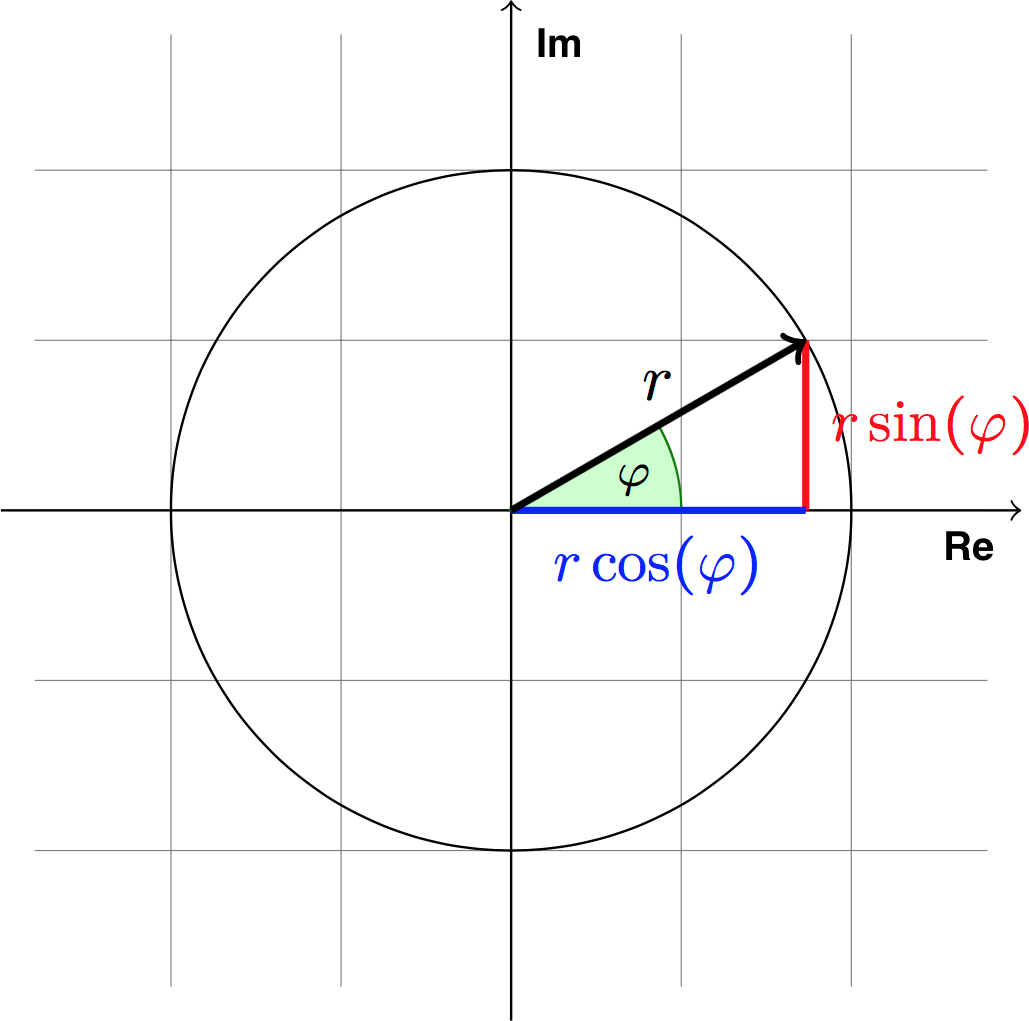
\includegraphics[width=\linewidth,keepaspectratio=true]{images/polarform}
\end{minipage}
%
\begin{minipage}[c]{0.5\textwidth}
\begin{equation*}
\begin{split}
	z & = x + iy = r(\cos(\varphi) + i\sin(\varphi)) = re^{i\varphi} \\
	r & = |z| = \sqrt{x^2 + y^2} \\
	\arg(z) & = \varphi  = \arctan(\frac{y}{x}) \quad \text{(je nach Quadrant)}  \\
	x & = r\cos(\varphi) \\
	y & = r\sin(\varphi) \\
	zw & = (re^{i\varphi})\cdot(se^{i\psi}) = rse^{i(\varphi + \psi)} \\
	\sqrt[q]{z} & = \sqrt[q]{s}e^{i\phi}\text{, wobei }\phi = \frac{\varphi}{q} \mod \frac{2\pi}{q} \\
	e^{i(\frac{\pi}{2} + 2\pi k)} & = i,\ e^{i\pi} = 1, \ e^{-i\pi} = -1
\end{split}
\end{equation*}
\end{minipage}

\begin{minipage}[c]{0.5\textwidth}
\begin{equation*}
\begin{split}
	(a,b) \cdot (c, d) & = (ac-bd, ad+bc) \\
	\overline{z} & = x - iy\\
	z^{-1} & = \frac{\overline{z}}{|z|^2} \\
	i & = \sqrt{-1}\\
\end{split}
\end{equation*}
\end{minipage}
%
\begin{minipage}[c]{0.5\textwidth}
\begin{equation*}
\begin{split}
	i^2 & = -1 \\
	|z|^2 & = z\overline{z} \\
	|zw|^2 & = (zw) \cdot \overline{(zw)} = |z|^2|w|^2
\end{split}
\end{equation*}
\end{minipage}

\section{Grenzwert}

\subsection{Dominanz}

\begin{equation*}
\begin{split}
	\text{F{\"u}r}\ x \to +\infty:\quad & ... < \log(\log(x)) < \log(x) < x^\alpha < \alpha^x < x! < x^x \\
	\text{F{\"u}r}\ x \to 0:\quad & ... < \log(\log(x)) < \log(x) < (\frac{1}{x})^\alpha \\
\end{split}
\end{equation*}

\subsection{Fundamentallimes}

\begin{equation*}
\begin{split}
	\lim_{x \to a} \frac{\sin \odot}{\odot} = \lim_{x \to a} \frac{\tan \odot}{\odot} & = 1\ \text{mit}\ \odot \xrightarrow{\: x \to a \: } 0 \\ 
	\lim_{x \to a} (1 + \frac{1}{\odot})^\odot & = e\ \text{mit}\ \odot \xrightarrow{\: x \to a \: } \infty \\ 
	\lim_{x \to a} (1 + \odot)^\frac{1}{\odot} & = e\ \text{mit}\ \odot \xrightarrow{\: x \to a \: } 0 \\ 
\end{split}
\end{equation*}

\subsection{Wurzeltrick}

\begin{equation*}
	\lim_{x\to\infty} \sqrt{\alpha}+\beta = \lim_{x\to\infty}(\sqrt{\alpha}+\beta)\frac{\sqrt{\alpha}-\beta}{\sqrt{\alpha}-\beta}
\end{equation*}

\subsection{$e^{\log(x)}$-Trick}

\paragraph{Anforderung:}Term der Form $f(x)^{g(x)}$ mit Grenzwert "$0^0$", "$\infty^0$" oder "$1^\infty$" f{\"u}r $x \to 0$

\begin{equation*}
	\textbf{Grundsatz:}\quad\lim_{x\to a}f(x)^{g(x)} = \lim_{x\to a}e^{g(x) \cdot \log(f(x))}
\end{equation*}

\emph{Tipp:} Danach den Limes des Exponenten berechnen. Oft ist Bernoulli-de l'H{\^o}pital dazu n{\"u}tzlich.

\subsection{Substitution}

\begin{equation*}
\begin{split}
	\lim_{x\to \infty} x^2(1 - \cos(\frac{1}{x})) \Rightarrow u = \frac{1}{x} \Rightarrow \lim_{x\to 0} \frac{1 - \cos(u)}{u^2}
\end{split}
\end{equation*}

\subsection{Satz von Bernoulli-de l'H{\^o}pital}

\paragraph{Anforderung:}Term der Form $\frac{f(x)}{g(x)}$ mit Grenzwert entweder "$\frac{0}{0}$" oder "$\frac{\infty}{\infty}$" mit $g'(x) \neq 0$. \\

\begin{equation*}
	\textbf{Grundsatz:}\quad\lim_{x\to a}\frac{f(x)}{g(x)} = \lim_{x\to a}\frac{f'(x)}{g'(x)}
\end{equation*}

\begin{table}[H]
\centering
\begin{tabular}{|c|c|c|}
\hline
\textbf{Term} & \textbf{Anforderung} & \textbf{Umformung} \\ \hline
$f(x)g(x)$              & "$0\cdot\infty$"                     & $\frac{g(x)}{\frac{1}{f(x)}}$          \\ \hline 
$\frac{f(x)}{g(x)} - \frac{h(x)}{i(x)}$ & "$\infty - \infty$"  & $\frac{f(x)i(x) - h(x)g(x)}{g(x)i(x)}$ \\ \hline      
\end{tabular}
\end{table}

\subsection{Wichtige Grenzwerte}

\begin{equation*}
\begin{split}
	\lim\limits_{n \to \infty} \left( 1+\frac{x}{n} \right)^n = e^x \qquad & \qquad \lim\limits_{n \to \infty} \left( 1+\frac{1}{n} \right)^n = e \\
	\lim\limits_{x \to 0} \frac{a^x-1}{x} = \ln a \qquad & \qquad \lim\limits_{x \to 0} \frac{\log_a(1+x)}{x} = \frac{1}{\ln a} \\
	\lim\limits_{x \to 0} \frac{1-\cos(x)}{x} = 0 \quad \qquad & \qquad \lim\limits_{x \to 0} \frac{1-\cos(x)}{x^2} = \frac{1}{2} \\
	\lim\limits_{x \to 0} \frac{\tan(x)}{x} = 1 \qquad & \qquad \lim\limits_{x \to 0} \frac{\sin(x)}{x} = 1 \\
	\lim\limits_{n \to \infty} \frac{n!}{n^n} = 0 \qquad & \qquad \lim\limits_{n \to 0} \frac{e^n -1 }{n} = 1 \\
	\lim\limits_{n \to \infty} \sqrt[n]{n!} = \infty \qquad & \qquad \lim\limits_{n \to \infty} \sqrt[n]{n} = 1 \\
	\lim\limits_{n \to \infty} \ln(n) = \infty \qquad & \qquad \lim\limits_{x \to 0} \frac{\log_a(1+x)}{x} = \frac{1}{\ln a} \\
\end{split}
\end{equation*}

\section{Folgen}

\subsection{Definition}

\begin{equation*}
\begin{split}
	\textbf{Konvergenz:} \quad & \forall \varepsilon > 0\ \exists N = N(\varepsilon) \in \mathbb{N},\ \text{sodass}\ \forall n \geq N: |a_n - a| < \varepsilon \\
	\textbf{Divergenz:} \quad & \forall K > 0\ \exists N = N(K) \in \mathbb{N},\ \text{sodass}\ \forall n \geq N: |a_n| > K
\end{split}
\end{equation*}

\subsection{Beweis}

\begin{enumerate}[noitemsep]
	\item Zeige mittels \textbf{Induktion}, dass die Folge \textbf{beschr{\"a}nkt} ist und monoton \textbf{steigt/f{\"a}llt}. Benutze dazu z.B. folgende Aussagen: $a_n \leq a_{n+1}$ oder $a_{n+1}-a_n \geq 0$.
	\item \textbf{Grenzwert berechnen} mit $a := \lim_{n \to \infty} a_n$ oder durch die ersten paar Terme absch{\"a}tzen
	\item Beweise den Grenzwert (z.B. mit $a_n \geq a$) um Beschr{\"a}nktheit zu beweisen
\end{enumerate}

\emph{Tipp:} Den Grenzwert in der rekursiven Formel mit $a_n$ und $a_{n+1}$ ersetzen. \\
F{\"u}r die Formel $a_{n+1} = \frac{1}{2}a_n + \sqrt{a_n}$ muss zum Beispiel gelten: $a = \frac{1}{2}a + \sqrt{a}$ (hier $a = 4$)

\section{Reihen $\sum^\infty$}

\subsection{Konvergenzkriterien}

\begin{table}[H]
\centering
\begin{tabular}{|p{4.5cm}|p{3.5cm}|p{4.3cm}|}
\hline
                                             & \textbf{Eignung}    & \textbf{Bemerkung}                        \\ \hline
\textbf{Limes des allgemeinen Glieds}        &                     & zeigt nur Divergenz                       \\ \hline
\textbf{Majoranten- und Minorantenkriterium} &                     & ersten Glieder spielen keine Rolle        \\ \hline
\textbf{Quotientenkriterium}                 & $a_n$ mit Faktoren wie $n!$, $a^n$, oder Polynome & gleiche Folgerung wie Wurzelkriterium     \\ \hline
\textbf{Wurzelkriterium}                     & $a_n = (b_n)^n$     & gleiche Folgerung wie Quotientenkriterium \\ \hline
\textbf{Leibnitz-Kriterium}                  & $\sin$, $\cos$, $\tan$, $(-1)^n$ &                                           \\ \hline
\textbf{Absolute Konvergenz}                 & $\sin$, $\cos$, $\tan$, $(-1)^n$   &                                           \\ \hline
\textbf{Sandwich-Theorem}					 & $\sin$, $\cos$, $\tan$, $(-1)^n$ & \\ \hline
\end{tabular}
\end{table}

\clearpage

\subsubsection*{Limes des allgemeinen Glieds}

\paragraph{Bemerkung:} Mit dieser Methode l{\"a}sst sich nur die Divergenz beweisen, nicht jedoch die Konvergenz.

\begin{enumerate}
	\item $\sum_n a_n$ gegeben
	\item Grenzwert $\lim_{n\mapsto\infty} a_n$ berechnen
	\begin{itemize}
		\item falls Grenzwert $\neq 0 \Rightarrow$ \textbf{divergent} 
		\item falls Grenzwert $= 0 \Rightarrow$ keine Aussage 
	\end{itemize}
\end{enumerate}

\subsubsection*{Majoranten- und Minorantenkriterium}

Es seien $a_n$, $b_n > 0$ mit $a_n \geq b_n\ \forall n$ ab einem gewissen $n_0$. Dann gilt: 
\begin{equation*}
\begin{split}
	\sum_n a_n \text{ konvergent} & \Rightarrow \sum_n b_n \textbf{ konvergent}\quad \text{(Majorantenkriterium)} \\
	\sum_n b_n \text{ divergent} & \Rightarrow \sum_n a_n \textbf{ divergent}\quad \text{(Minorantenkriterium)} \\
\end{split}
\end{equation*}

\subsubsection*{Vergleichskriterium}

\begin{enumerate}
	\item $\sum_n a_n$ und $\sum_n b_n$ gegeben mit $a_n,b_n > 0$
	\item Grenzwert $\lim_{n\mapsto\infty} \frac{a_n}{b_n}$ berechnen
	\begin{itemize}
		\item falls Grenzwert $= 0$:
		\begin{itemize}
			\item $\sum_n a_n$ divergent $\Rightarrow \sum_n b_n$ \textbf{divergent}
			\item $\sum_n b_n$ konvergent $\Rightarrow \sum_n a_n$ \textbf{konvergent}
		\end{itemize} 
		\item falls Grenzwert $= \infty$:
		\begin{itemize}
			\item $\sum_n a_n$ konvergent $\Rightarrow \sum_n b_n$ \textbf{konvergent}
			\item $\sum_n b_n$ divergent $\Rightarrow \sum_n a_n$ \textbf{divergent}
		\end{itemize} 
	\end{itemize}
\end{enumerate}

\subsubsection*{Quotientenkriterium}

\begin{enumerate}
	\item $\sum_n a_n$ mit $a_n \neq 0$ gegeben
	\item Grenzwert $\lim_{n\mapsto\infty}|\frac{a_{n+1}}{a_n}|$ berechnen
	\begin{itemize}
		\item falls Grenzwert $> 1 \Rightarrow$ \textbf{divergent}
		\item falls Grenzwert $< 1 \Rightarrow$ \textbf{konvergent}
		\item falls Grenzwert $= 1 \Rightarrow$ keine Aussage
	\end{itemize}
\end{enumerate}

\subsubsection*{Wurzelkriterium}

\begin{enumerate}
	\item $\sum_n a_n$ mit $a_n \neq 0$ gegeben
	\item Grenzwert $\lim_{n\mapsto\infty}\sqrt[n]{|a_n|}$ berechnen
	\begin{itemize}
		\item falls Grenzwert $> 1 \Rightarrow$ \textbf{divergent}
		\item falls Grenzwert $< 1 \Rightarrow$ \textbf{konvergent}
		\item falls Grenzwert $= 1 \Rightarrow$ keine Aussage
	\end{itemize}
\end{enumerate}

\subsubsection*{Leibniz-Kriterium}

\begin{enumerate}
	\item $\sum_n (-1)^n a_n$ gegeben
	\item \textbf{konvergent}, falls:
	\begin{enumerate}
		\item $a_n \geq 0$
		\item $\lim_{n\mapsto\infty} a_n = 0$
		\item $a_n$ monoton fallend
	\end{enumerate}
\end{enumerate}

\subsubsection*{Absolute Konvergenz}

\begin{enumerate}
	\item $\sum_n (-1)^n a_n$ gegeben
	\item \textbf{konvergent}, falls $\sum_n |a_n|$ konvergent
\end{enumerate}

\subsection{Geometrische Reihe}

Reihe der Form $\sum^\infty_{k = 0} a \cdot r^k$ mit der \textbf{Partialsumme}:

\begin{equation*}
	S_N=\frac{a-ar^{N+1}}{1-r}
\end{equation*}

\textbf{Konvergent}, falls $0<|r|<1$ mit Grenzwert:

\begin{equation*}
	\sum^\infty_{k=0}ar^k=\frac{a}{1-r}
\end{equation*}

\subsection{Potenzreihe}

Reihe der Form $\sum^\infty_0 a_nx^n$. \textbf{Konvergent}, falls $|x|<\rho$. In diesem Gebiet darf man die Reihe ableiten und integrieren.

\begin{equation*}
	\rho= \lim_{n\rightarrow \infty}|\frac{a_n}{a_{n+1}}|
\end{equation*}
\begin{equation*}
	\rho=\frac{1}{\lim_{n\rightarrow \infty}\sqrt[n]{|a_n|}}
\end{equation*}

\paragraph{Konvergenzverhalten am Rand:} Es muss noch {\"u}berpr{\"u}ft werden, ob die Reihe f{\"u}r genau $\rho$ konvergiert. Dazu muss $\rho$ in die Formel eingesetzt werden.

\subsubsection{Wichtige Reihen}

\renewcommand{\arraystretch}{1.5}
\begin{table}[H]
	
	\begin{tabular}{l|l}
		$\cos(x)$ & $\sum^\infty_{n =0}\frac{(-1)^nx^{2n}}{(2n)!}$ \\\hline
		$\sin(x)$ & $\sum^\infty_{n =0}\frac{(-1)^nx^{2n+1}}{(2n+1)!}$ \\ \hline
		$e^x$ & $\sum^\infty_{n =0}\frac{x^n}{n!} $\\\hline
		$n^2$ & $\sum_{k=1}^n 2k-1$        \\\hline
		$\sum_{n=1}^{\infty}\frac{1}{n}$ & $harmonisch$
	\end{tabular}
\end{table}


\subsubsection{Potenzreihenentwicklung}

\begin{equation*}
	\textbf{Grundsatz:} \quad f(x) = \sum_{n=0}^\infty \frac{f^{(n)}(0)}{n!} \cdot x^n
\end{equation*}

\section{Stetigkeit}

\subsection{Lipschitz-Stetigkeit}
Es existiert eine Konstante $L\in \mathbb{R}$, sodass:
\begin{equation*}
	|f(x)-f(y)|\leq L|x-y| \quad \forall x,y \in \Omega
\end{equation*}

\emph{Bemerkung:} Ist $f'$ \textbf{auf $\Omega$ beschr{\"a}nkt}, so ist $f$ Lipschitz-stetig. Lipschitz-Stetigkeit impliziert gleichm{\"a}ssige Stetigkeit.

\subsection{Weierstrass-Kriterium}
F{\"u}r alle $\epsilon > 0$ gibt es ein $\delta(\epsilon, a) >0$, sodass f{\"u}r alle $|x-a|<\delta$ gilt:
\begin{equation*}
	|f(x) -f(a)|<\epsilon
\end{equation*}

\subsection{Gleichm{\"a}ssige Stetigkeit}
F{\"u}r alle $\epsilon > 0$ gibt es ein $\delta(\epsilon) >0$, sodass f{\"u}r alle $|x-y|<\delta$ gilt:
\begin{equation*}
	|f(x)-f(y)| < \epsilon
\end{equation*}
\emph{Bemerkung:} Ist $f$ \textbf{stetig und kompakt}, dann ist sie auch gleichm{\"a}ssig stetig.

\subsection{Punktweise Konvergenz}

$f_n(x)$ konvergiert punktweise falls:
\begin{equation*}
	\forall x\in \Omega \quad \lim_{n\rightarrow\infty}f_n(x) = f(x)
\end{equation*}

\subsection{Gleichm{\"a}ssige Konvergenz}

\paragraph{Grundsatz:} Falls eine Folge stetiger Funktionen $f_n$ gleichm{\"a}ssig gegen $f$ konvergiert, muss $f$ stetig sein.\\

$f_n(x)$ konvergiert gleichm{\"a}ssig falls:
\begin{equation*}
	\lim_{n\rightarrow\infty} \sup|f_n(x) - f(x)| = 0
\end{equation*}

\emph{Bemerkung:} Gleichm{\"a}ssige Konvergenz impliziert punktweise Konvergenz.\\
\underline{Rezpet f{\"u}r gleichm{\"a}ssige Konvergenz} 
\begin{enumerate}[label=(\roman*)]
	\item Punktweiser Limes berechnen
				\[
						\lim_{n\rightarrow\infty}f_n(x) = f(x) \text{\quad = Grenzfunktion}
				\]
	\item Supremum bestimmen \\
				(Ableitung von $f_n(x)$  oder Absch{\"a}tzung benutzen)
				\[
						\sup|f_n(x) - f(x)|
				\]
	\item Limes $n \to \infty$ bestimmen (vgl. Kriterium glm. Konvergenz)
				\[
						\lim_{n\rightarrow\infty} \sup|f_n(x) - f(x)|
				\]
				Limes = 0 $\rightarrow$ Glm. konvergent mit Grenzfunktion f(x)
	\item Indirekte Methode \\
				\begin{itemize}
					\item $f(x)$ unstetig  auf $\Omega \Rightarrow$ keine glm. Konvergenz	
					\item $f(x)$ stetig, $f_n(x) \leq f_{n+1}(x) \forall x \in \Omega $ und $\Omega$ kompakt $\Rightarrow$ Glm. Konvergenz
				\end{itemize}

\end{enumerate}

\begin{equation*}
\begin{split}
	\text{gegeben:} \quad & f_n:[0,1] \mapsto \mathbb{R},\ f_n(x) = (1 - x^2)x^n \\
	\textbf{punktweisen Limes berechnen:} \quad & \lim_{n \to \infty} (1 - x^2)x^n = 0 \equiv f(x) \\
	& \Rightarrow\ \text{konvergiert gegen 0} \\
	\text{Supremum berechnen:} \quad & \sup_{x \in [0,1]} |f_n(x) -f(x)| = \sup_{x \in [0,1]} |f_n(x)| = \sup_{x \in [0,1]}f_n(x) \\
	\text{Maximum finden:} \quad & \frac{d}{dx} f_n(x) nx^{n-1}(1-x^2)-2xx^n = x^{n-1}(n - (n+2)x^2) = 0 \\
	& \Rightarrow x_1 = 0,\ x_2 = \sqrt{\frac{n}{n+2}} \Rightarrow x_2\ \text{ist Maximum} \\
	\textbf{Limes berechnen:} \quad & \lim_{n \to \infty} \sup_{x \in [0,1]} |f_n(x) - f(x)| = \lim_{n \to \infty} f_n(x_2) = 0 \\
	\textbf{Folgerung:} \quad & \text{$f_n$ konvergiert auf $[0,1]$ glm. gegen $f$}
\end{split}
\end{equation*}

\section{Differenzialrechnung}

Eine stetige Funktion ist differenzierbar, falls der Grenzwert $f'(x_0)$ existiert:

\begin{equation*}
	f'(x_0) := \lim_{x\to x_0}\frac{f(x) - f(x_0)}{x-x_0}
\end{equation*}
\subsubsection*{Tangente}
		Sei $f: \Omega \to \mathbb{R}$ an der Stelle $x_0 \in \Omega$ diffbar. Dann ist die Tangente im Punkt $x_0$
		\[ t(x; x_0)=f(x_0)+f'(x_0)(x-x_0) \]

\subsection{Umkehrsatz}

\begin{equation*}
	(f^{-1})'(y) = \frac{1}{f'(f^{-1}(y))}
\end{equation*}

\subsection{Mittelwertsatz}

\begin{equation*}
	f'(c) = \frac{f(b) - f(a)}{b - a}
\end{equation*}

\subsection{Taylorpolynom}

Das Taylorpolynom $m$-ter Ordnung von $f(x)$ an der Stelle $x=a$
\begin{equation*}
	P^a_m(x) := f(a) + f'(a)(x-a) + \frac{1}{2}f''(a)(x-a)^2 + ... + \frac{1}{m!} f^{(m)}(a)(x-a)^m
\end{equation*}

mit dem Fehlerterm $R^a_m(x)$, wobei $\xi$ zwischen $a$ und $b$ liegt:
\begin{equation*}
	R^a_m(x) = \frac{f^{(m+1)}(\xi)}{(m+1)!}(x+a)^{m+1},\ \text{wobei}\ f(x) = P^a_m(x) + R^a_m(x)
\end{equation*}

\subsection{Hauptsatz der Differential- und Integralrechnung}

\begin{equation*}
	f(x)=\int^{m(x)}_lg(t)dt
\end{equation*}
\begin{equation*}
	f'(x)=g(m(x))\cdot\frac{d}{dx}m(x)
\end{equation*}
wobei $m(x)$ der Form $ax^b$ ist mit $l\in \mathbb{R}$\\\\
\underline{Differenzial / Jaccobi-Matrix}
		\begin{equation*}
				df = 
					\begin{pmatrix}
						\frac{\partial f_1}{\partial x_1} & ... & \frac{\partial f_1}{\partial x_n} \\
						... & ... & ... \\
						\frac{\partial f_m}{\partial x_1} & ... & \frac{\partial f_m}{\partial x_n}
					\end{pmatrix}
		\end{equation*}
		$\rightarrow$ enth{\"a}lt die $n$ part. Ableit. aller m Komponenten von $f$\\
\subsubsection*{Taylorentwicklung mit mehreren Variabeln} 
	\begin{tabular}{ll}
		$f(x,y) =  $ & $f(x_0,y_0) + \frac{\partial f}{\partial x} \Delta x + \frac{\partial f}{\partial y} \Delta y$ \\
			& $ + \frac{1}{2!} \bigg{(}
						 \frac{\partial^2 f}{\partial x^2} (\Delta x)^2	
						 + 2\frac{\partial^2 f}{\partial x \partial y} \Delta x \Delta y 
						 + \frac{\partial^2 f}{\partial y^2} (\Delta y)^2	
									\bigg{)} $ \\
			& $ + \frac{1}{3!} \bigg{(}
						 \frac{\partial^3 f}{\partial x^3} (\Delta x)^3
						 + 3\frac{\partial^3 f}{\partial x^2 \partial y} (\Delta x)^2 \Delta y$ \\
			&			\qquad  $+ 3\frac{\partial^3 f}{\partial x \partial y^2} \Delta x (\Delta y)^2 
						 + \frac{\partial^3 f}{\partial y^3} (\Delta y)^3
						\bigg{)} $ \\
			& 			$+ \cdots$			
	
	\end{tabular}

\section{Integration}

\subsection{Elementare Integrale}

\begin{table}[H]
\centering
\begin{tabular}{|c|c|c|}
\hline
$f'(x)$ & $f(x)$ & $F(x)$ \\ \specialrule{.1em}{0em}{0em} 
$\frac{f'(x)g(x) - f(x)g'(x)}{g(x)^2}$ & $\frac{f(x)}{g(x)}$ &  \\ \hline
$0$ & $c$ & $cx$ \\ \hline
$r\cdot x^{r-1}$ & $x^r$ & $\frac{x^{r+1}}{r+1}$ \\ \hline
$-\frac{1}{x^2} = -x^{-2}$ & $\frac{1}{x} = x^{-1}$ & $\ln|x|$ \\ \hline
$\frac{1}{2\sqrt{x}} = \frac{1}{2}x^{-\frac{1}{2}}$ & $\sqrt{x} = x^{\frac{1}{2}}$ & $\frac{2}{3}x^\frac{3}{2}$ \\ \hline
$\cos(x)$ & $\sin(x)$ & $-\cos(x)$ \\ \hline
$-\sin(x)$ & $\cos(x)$ & $\sin(x)$ \\ \hline
$1 + \tan^2(x) = \frac{1}{\cos^2(x)}$ & $\tan(x)$ & $-\ln|\cos(x)|$ \\ \hline
$e^x$ & $e^x$ & $e^x$ \\ \hline
$c\cdot e^{cx}$ & $e^{cx}$ & $\frac{1}{c}\cdot e^{cx}$ \\ \hline
$\ln(c)\cdot c^x$ & $c^x$ & $\frac{c^x}{\ln(c)}$ \\ \hline
$\frac{1}{x}$ & $\ln|x|$ & $x(\ln|x| - 1)$ \\ \hline
$\frac{1}{\ln(a) \cdot x}$ & $\log_a|x|$ & $\frac{x}{\ln(a)}(\ln|x| -1)$ \\ \hline
$\frac{1}{\sqrt{1-x^2}}$ & $\arcsin(x)$ & $x\cdot\arcsin(x) + \sqrt{1-x^2}$ \\ \hline
$-\frac{1}{\sqrt{1-x^2}}$ & $\arccos(x)$ & $x\cdot\arccos(x) - \sqrt{1-x^2}$ \\ \hline
$\frac{1}{1+x^2}$ & $\arctan(x)$ & $x\cdot \arctan(x) - \frac{1}{2}\ln(1+x^2)$ \\ \hline
$\cosh(x)$ & $\sinh(x) = \frac{e^x - e^{-x}}{2}$ & $\cosh(x)$ \\ \hline
$\sinh(x)$ & $\cosh(x) = \frac{e^x + e^{-x}}{2}$ & $\sinh(x)$ \\ \hline
$\frac{1}{\cosh^2(x)}$ & $\tanh(x)$ & $\log(\cosh(x))$ \\ \hline
\end{tabular}
\end{table}

\subsection{Regeln}

\begin{equation*}
\begin{split}
	\textbf{Direkter Integral}\quad & \int f(g(x))g'(x)\ dx = F(g(x)) \\
	\textbf{Partielle Integration}\quad & \int f' \cdot g\ dx = f \cdot g - \int f \cdot g'\ dx \\
	\textbf{mit Polynomen}\quad & \int\frac{p(x)}{q(x)}\ dx \Rightarrow\ \text{Partialbruchzerlegung} \\
	\textbf{Substitution}\quad & \int_a^b f(\varphi(t))\varphi'(t)\ dt = \int_{\varphi(a)}^{\varphi(b)} f(x)\ dx\ \text{mit}\ x = \varphi(t)
\end{split}
\end{equation*}

\subsection{Tipps}

\begin{equation*}
\begin{split}
	\int\tan x\ dx & = \int\frac{\sin x}{\cos x}\ dx = -\log|\cos(x)| \\
	\int \frac{1}{x - \alpha}\ dx & = \log(x-\alpha) \\
	\int\frac{\frac{1}{\alpha}}{1+(\frac{x}{\alpha})^2}\ dx & = \arctan(x) \\
	\int \sin^2(x)\ dx & = \frac{1}{2}(x - \sin(x)\cos(x)) + C \\
	\int \cos^2(x)\ dx & = \frac{1}{2}(x + \sin(x)\cos(x)) + C \\
	\int \sqrt{x^2+1}\ dx & = \sinh(x) + C
\end{split}
\end{equation*}

\subsection{Uneigentliche Integrale}

\begin{equation*}
\begin{split}
	\int_0^\infty f(x)\ dx = \lim_{R \to \infty} \int_0^R f(x)\ dx \\
	\int_{-\infty}^\infty f(x)\ dx = \lim_{R \to -\infty} \int_R^k f(x)\ dx + \lim_{R \to \infty} \int_k^R f(x)\ dx
\end{split}
\end{equation*}

Gibt es eine Unstetigkeitstelle $c$ in dem Integrationsgebiet, so geht man wie folgt vor:
\begin{equation*}
	\int_a^b f(x)\ dx = \lim_{\varepsilon \to 0} \int_a^{c-\varepsilon} f(x)\ dx + \lim_{\varepsilon \to 0} \int_{c+\varepsilon}^b f(x)\ dx
\end{equation*}

\subsection{Beweis bijektiver Funktionen}

Zu beweisen sind folgende Eigenschaften:
\begin{description}[labelindent=16pt,style=multiline,leftmargin=3cm, noitemsep]
	\item[injektiv:] Zeig, dass $f$ \textbf{strickt monoton w{\"a}chst oder f{\"a}llt} und\textbf{stetig} ist
	\item[surjektiv:] Zeig, dass alle Werte im Bildbereich angenommen werden (vl. mit Zwischenwertsatz)
\end{description}
Daraus folgt dann, dass $f$ bijektiv ist.

\section{Differentialgleichungen}

\subsection{Grundbegriffe}

\begin{description}[labelindent=16pt,style=multiline,leftmargin=3.5cm, noitemsep]
	\item[Ordnung:] h{\"o}chste vorkommende Ableitung
	\item[linear:] alle $y$-abh{\"a}ngigen Terme kommen linear vor (keine Terme wie zum Beispiel $y^2$, $(y'')^3$, $\sin(y)$, $e^{y'}$)
	\item[homogen:] Gleichung ohne St{\"o}rfunktionen
	\item[St{\"o}rfunktion:] Term, der rein von der Funktionsvariablen $x$ abh{\"a}ngt
\end{description}

\subsection{Methoden}

\begin{table}[H]
\centering
\begin{tabular}{|p{3cm}|p{6cm}|p{3cm}|}
\hline
                                  	& \textbf{Problem} 							& \textbf{Anforderungen} 			\\ \hline
\textbf{Trennung der Variablen}   	& $y' = \frac{dy}{dx} = h(x) \cdot g(y)$ 	& 1. Ordnung			            \\ \hline
\textbf{Variation der Konstanten}	& $y' = \frac{dy}{dx} = h(x)y + b(x)$	 	& 1. Ordnung \filbreak inhomogen	\\ \hline
\textbf{Euler-Ansatz}				& $a_{n}y^{(n)} + a_{n-1}y^{(n-1)} + ... + a_{0}y = 0$	 	& n. Ordnung \filbreak linear \filbreak homogen	\\ \hline
\textbf{Direkter Ansatz}				& $a_{n}y^{(n)} + a_{n-1}y^{(n-1)} + ... + a_{0}y = b(x)$	& n. Ordnung \filbreak linear \filbreak inhomogen	\\ \hline

%\textbf{Substitution}				& $y' = h(\frac{y}{x})$ \filbreak $y' = h(ax + by + c)$ \filbreak $y' = h(\frac{ax + by + c}{dx + ey + f})$ \filbreak $y' = \frac{y}{x}h(xy)$ 																		& nicht direkt separierbar			\\ \hline
\end{tabular}
\end{table}

\subsubsection{Trennung der Variable}

\begin{equation*}
\begin{split}
	& y' + x \tan y = 0,\ y(0) = \frac{\pi}{2} \\
	\text{umformen}\quad & \frac{dy}{dx} = -x \tan y \\
	\textbf{konstante L{\"o}sungen}\quad & y(x) \equiv 0\ \text{erf{\"u}llt jedoch $y(0) \equiv \frac{\pi}{2}$ nicht} \\
	\text{Trennung}\quad & \frac{dy}{\tan y} = -x dx \\
	\text{integrieren}\quad & \int\frac{\cos y}{\sin y}dy = - \int xdx \Rightarrow \log|\sin y| = -\frac{x^2}{2} + C \\
	& \Rightarrow |\sin y| = e^Ce^{\frac{-x^2}{2}} \Rightarrow \sin y = \pm e^Ce^{\frac{-x^2}{2}} = Ce^{\frac{-x^2}{2}} \\
	\text{Anfangsbedingung gebrauchen}\quad & \sin(y(0)) = \sin (\frac{\pi}{2}) = 1 \Rightarrow C = 1 \\
	\textbf{L{\"o}sung}\quad & y(x) = \arcsin (e^{\frac{-x^2}{2}})
\end{split}
\end{equation*}

\clearpage

\subsubsection{Variation der Konstanten}

\begin{equation*}
	\textbf{Grundsatz:}\quad y(x) = y_h(x) + y_p(x)
\end{equation*}

\begin{equation*}
\begin{split}
	& y'(x+1) + y = x^3,\ y(0) = \sqrt{5} \\
	\text{Trennung}\quad & \frac{y'}{y} = \frac{-1}{x+1} \\
	\textbf{konstante L{\"o}sungen}\quad & y(x) \equiv 0\ \text{erf{\"u}llt jedoch $y(0) \equiv \sqrt{5}$ nicht} \\
	\text{integrieren}\quad & \int \frac{dy}{y} = - \int \frac{dx}{x+1} \\
	& \Rightarrow \ln|y| = -\ln|x+1| + C \\
	\textbf{Homogene L{\"o}sung} \quad & y_h(x) = \frac{C}{x+1},\ \text{mit}\ C= \pm e^C \in \mathbb{R}\backslash{0} \\
	\text{partikul{\"a}rer Ansatz}\quad & y_p(x) = \frac{C(x)}{x+1} \\
	\text{einsetzen} \quad & (\frac{C'(x)}{x+1} - \frac{C(x)}{(x+1)^2})(x+1) + \frac{C(x)}{x+1} = x^3 \\
	& C'(x) = x^3 \\
	& C(x) = \frac{x^4}{4} \\
	\textbf{partkul{\"a}re L{\"o}sung} \quad & y_p(x) = \frac{x^4}{4(x+1)} \\
	\text{allgemeine L{\"o}sung}\quad & y(x) = y_h(x) + y_p(x) = \frac{C}{x+1} + \frac{x^4}{4(x+1)} \\
	\text{Anfangsbedingung benutzen} \quad & y(0) = \sqrt{5} \Rightarrow C = \sqrt{5} \\
	\textbf{L{\"o}sung} \quad & y(x) = \frac{\sqrt{5}}{x+1} + \frac{x^4}{4(x+1)}
\end{split}
\end{equation*}

%\subsubsection{Substitution}
%
%\begin{equation*}
%\begin{split}
%	& y' = h(\frac{y}{x})\ \text{ersetzt durch}\ z(x) = \frac{y(x)}{x} \Leftrightarrow y(x) = xz(x) \\
%	& \Rightarrow	y' = z + xz'
%\end{split}
%\end{equation*}



\subsubsection{Euler-Ansatz}

\begin{equation*}
\begin{split}
	& y'' - 2y' - 8y = 0,\ y(1) = 1, y'(1) = 0 \\
	\text{Euler-Ansatz}\quad & y(x) = e^{\lambda x} \\
	\text{einsetzen}\quad & \lambda^2 e^{\lambda x} - 2\lambda e^{\lambda x} - 8e^{\lambda x} = 0 \\
	\textbf{charakt. Polynom}\quad & \lambda^2 - 2\lambda - 8 = (\lambda - 4)(\lambda + 2) = 0 \\
	\text{Nullstellen}\quad & 4, -2 \\
	\textbf{allgemeine L{\"o}sung}\quad & y(x) = Ae^{4x} + Be^{-2x} \\
	\text{Anfangsbedingung gebrauchen}\quad & y(1) = Ae^4 + Be^{-2} =1,\\ &y'(1) = 4Ae^4 - 2Be^{-2} = 0 \\
											& \Rightarrow A = \frac{1}{3}e^{-4}, B = \frac{2}{3}e^2 \\
	\textbf{L{\"o}sung}\quad & y(x) = \frac{1}{3}e^{4x-4} + \frac{2}{3}e^{2-2x}
\end{split}
\end{equation*}

\emph{Bemerkung:} Zu einer $m$-fachen Nullstelle $\lambda$ geh{\"o}ren die $m$ linear unabh{\"a}ngigen L{\"o}sungen $e^{\lambda x}$, $x\cdot e^{\lambda x}$, ... , $x^{m-1}\cdot e^{\lambda x}$. Zur $m$-fachen Nullstelle $\lambda = 0$ geh{\"o}ren die L{\"o}sungen $1$, $x$, ... , $x^{m-1}$. \\
 
\emph{Komplexe Nullstellen:} \\

\begin{equation*}
	x = \frac{-b \pm \sqrt{b^2-4ac}}{2a}
\end{equation*}

Ein komplexes Nullstellenpaar der Form $\alpha \pm \beta i$ liefert folgende homogene L{\"o}sung:
\begin{equation*}
	y(x)=e^{\alpha x}(C_1\cos(\beta x) + C_2\sin(\beta x))
\end{equation*}



\subsubsection{Direkter Ansatz}

\begin{equation*}
	\textbf{Grundsatz:}\quad y(x) = y_\text{homo}(x) + y_p(x)
\end{equation*}

\begin{table}[H]
\centering
\begin{tabular}{|l|l|l|}
\hline
\textbf{Inhomogener Term $b(x)$} & \textbf{Ansatz f{\"u}r $y_p(x)$}	& \textbf{zu bestimmen}		\\ \hline
Polynom				& $Ax^2 + Bx + C$			& $A$, $B$, $C$		\\ \hline
$c e^{k x}$ & $Ae^{kx}$					& $A$				\\ \hline
$c\sin(kx)$ oder $c\cos(kx)$ & $A\sin(kx) + B\cos(kx)$ & $A$, $B$ \\ \hline

\end{tabular}
\end{table}

\emph{Bemerkung:} Kommt der gew{\"a}hlte Ansatz schon in der homogenen L{\"o}sung vor,\\ so multipliziert man den Ansatz einfach mit $x$.

\begin{equation*}
\begin{split}
	& y'' - y' + \frac{1}{4}y = \cos(x) \\
	\text{homogener Ansatz}\quad & y'' + y' + \frac{1}{4}y = 0 \\
	\text{Euler-Ansatz anwenden}\quad & \lambda^2 + \lambda + \frac{1}{4} = (\lambda + \frac{1}{2})^2 = 0 \\
	\textbf{homogene L{\"o}sung}\quad &\Rightarrow y_\text{homo}(x) = Ae^{-\frac{x}{2}} + Bx \cdot e^{-\frac{x}{2}} \\
	\text{partikul{\"a}rer Ansatz w{\"a}hlen}\quad & y_p(x) = a\cos(x) + b\sin(x) \\
							  & \Rightarrow y_p'(x) = -a\sin(x) + b\cos(x),\  y_p''(x) = \\ & = -a\cos(x) -b \sin(x) \\
	\text{Einsetzen}\quad & (-a + b + \frac{a}{4})\cos(x) + (-b -a + \frac{1}{4}b)\sin(x) = \cos(x) \\
	\text{Koeffizientenvergleich}\quad & -\frac{3}{4}a + b = 1,\ -a-\frac{3}{4}b = 0 \\
	\textbf{partikul{\"a}re L{\"o}sung}\quad & y_p(x) = -\frac{12}{25}\cos(x) + \frac{16}{25}\sin(x) \\
	\textbf{L{\"o}sung}\quad & y(x) = Ae^{-\frac{x}{2}} + Bx \cdot e^{-\frac{x}{2}} -\frac{12}{25}\cos(x) + \frac{16}{25}\sin(x)
\end{split}
\end{equation*}



% fill the page
%\clearpage


\end{document}


